\chapter{Resultat}\label{cha:Research}

\begin{figure}[H]
	\centering
	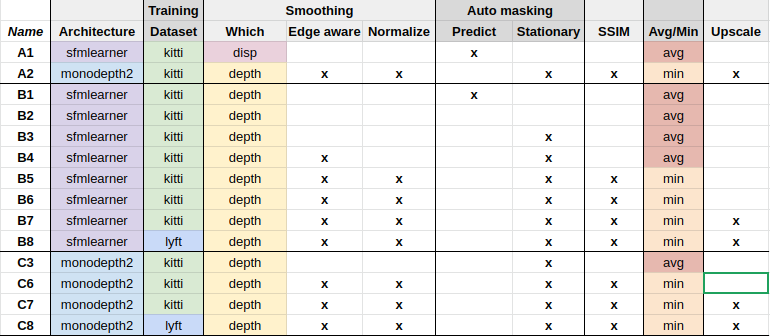
\includegraphics[width=1.0\textwidth]{configurations}
	\caption{Different configurations of network architecutes, training datasets and loss terms evaluated to find the best performance}
	\label{fig:conv}
\end{figure}

\begin{figure}[H]
	\centering
	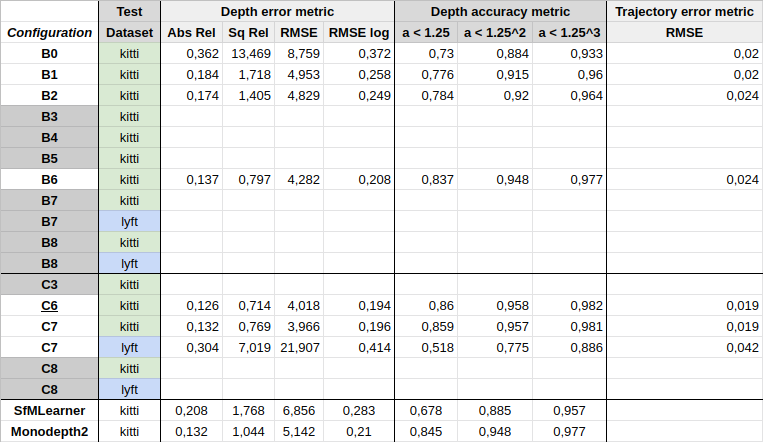
\includegraphics[width=1.0\textwidth]{evaluation}
	\caption{Evaluation metrics when testing the configurations on the testing split of the datasets}
	\label{fig:conv}
\end{figure}

\begin{figure}[H]
	\centering
	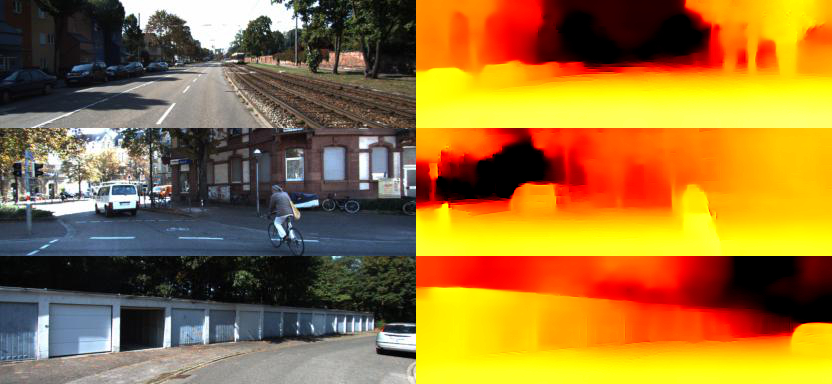
\includegraphics[width=1.0\textwidth]{depthmaps}
	\caption{Examples from the Kitti dataset}
	\label{fig:conv}
\end{figure}

\begin{figure}[H]
	\centering
	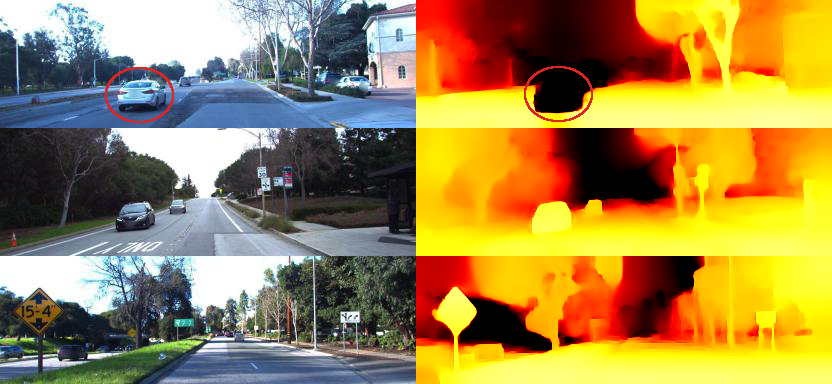
\includegraphics[width=1.0\textwidth]{depthmapslyft}
	\caption{Examples from the Lyft dataset}
	\label{fig:conv}
\end{figure}

\begin{figure}[H]
	\centering
	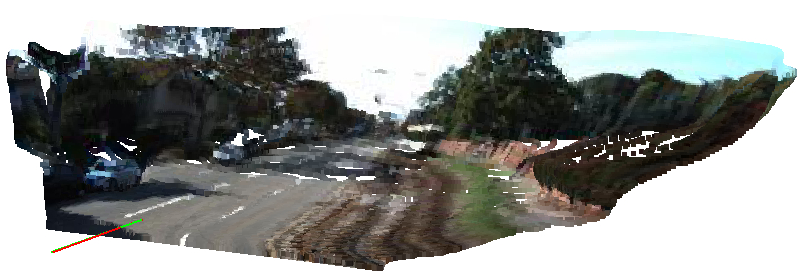
\includegraphics[width=1.0\textwidth]{3drender}
	\caption{3D render of colorized depth map}
	\label{fig:3drender}
\end{figure}

\begin{figure}[H]
	\centering
	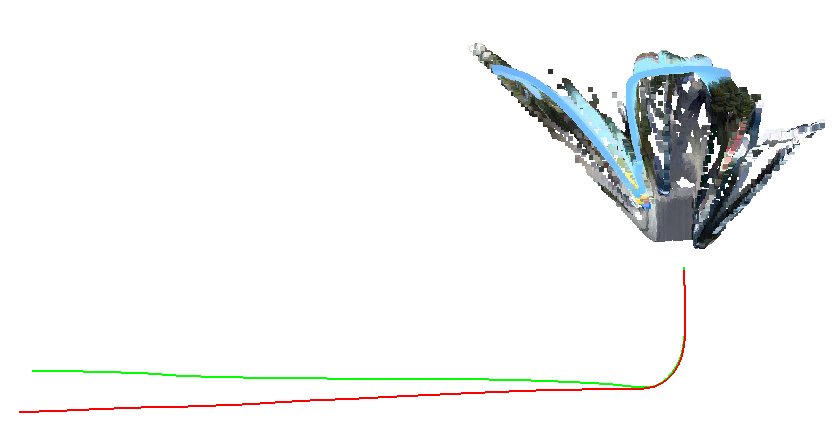
\includegraphics[width=1.0\textwidth]{movement}
	\caption{3D visualization of the camera movement in a long image sequence. The green line is ground truth and the red line is the predicted camera trajectory.}
	\label{fig:conv}
\end{figure}